\documentclass[12pt,a4paper]{report}

\usepackage[spanish]{babel}
\usepackage[utf8]{inputenc}
\usepackage{dad}

\title{Desarrollo de Aplicaciones Distribuidas: \\ Registrador de juegos}
\author{Rafael Gálvez-Cañero, Andreas Gerstmayr}
\date{Iteración 3 - 9 de Abril de 2015} % delete this line to display the current date



%%% BEGIN DOCUMENT
\begin{document}
\maketitle
\tableofcontents
\listoffigures
\listoftables

\pagenumbering{arabic}

% Esto representa la primera iteración (capítulo), información general
\chapter{Datos generales}

\section{Miembros del grupo}

\begin{table}[htdp]
\begin{center}
\begin{tabular}{|l|l|l|c|}
\hline
\textbf{Apellidos}&\textbf{Nombre}&\textbf{Correo-e}&\textbf{Grupo}\\
\hline
Gálvez-Cañero&Rafael&\href{mailto:galvesband@gmail.com}{galvesband@gmail.com}&18\\
Gerstmayr&Andreas&\href{mailto:andreas.gerstmayr@gmail.com}{andreas.gerstmayr@gmail.com}&18\\
\hline
\end{tabular}
\end{center}
\caption{Miembros del grupo}
\label{tab:miembros}
\end{table}%


\section{Descripción del sistema}

\begin{itemize}
\item \textbf{Tipo de sistema distribuido}: Sistema de información.
\item \textbf{Nombre del proyecto}: Plataforma de juegos, Game Registry.
\item \textbf{Breve descripción}: Sub-sistema para registrar sesiones de juego e información asociada.
\end{itemize}

\subsection{Funcionalidad observable}

\begin{itemize}
\item Registrar el inicio y el término de todas las sesiones de juego.
\item Visualizar el historial de juegos.
\end{itemize}

\subsection{Servicios ofrecidos}
\begin{itemize}
\item Servicio de Registro: Capacidad de aceptar la información de una sesión de juego (juego ID, jugador ID y fecha de inicio y término).
\item Servicio de Historial: Ofrece métodos para consultar el historial de sesiones.
\end{itemize}

\subsection{Servicios demandados}
\begin{itemize}
\item Servicio de Juego: avisar de término de una sesión de juego
\item Servicio de Juego: recibir el título de un juego
\item Servicio de Perfil: rebibir el nombre de un jugador
\end{itemize}

\section{Direcciones de descarga y planificación}

\begin{table}[htdp]
\begin{center}
\begin{tabular}{|c|c|}
\hline
\textbf{Código fuente}&\url{https://repositorio.informatica.us.es/svn/lq3vqrtzfnh2nx9yhpk}\\
\hline
\multicolumn{2}{|c|}{\textbf{Planificación temporal}}\\
\hline
Iteración 1&24/02/2015\\
Iteración 2&03/03/2015\\
Iteración 3&26/03/2015\\
Iteración 4&7/04/2015\\
Iteración 5&28/04/2015\\
Iteración 6&12/05/2015\\
Iteración 7&26/05/2015\\
Entrega Final&02/06/2015\\
\hline
\end{tabular}
\end{center}
\caption{Datos generales del trabajo en grupo}
\label{tab:datosgenerales}
\end{table}%

\section{Seguimiento}

\begin{table}[htdp]
\begin{center}
\begin{tabular}{|c|c|c|c|c|c|c|c|c|c|c|}
\cline{2-9}
\multicolumn{1}{c}{}&\multicolumn{8}{|c|}{\textbf{Iteración}}&\multicolumn{2}{c}{}\\
\hline
\textbf{Estudiante}&1&2&3&4&5&6&7&Final&Total&Pond.\\
\hline
Rafael Gálvez-Cañero&5&5&5&5&-&-&-&-&\textbf{20}&1\\
Andreas Gerstmayr   &5&5&5&5&-&-&-&-&\textbf{20}&1\\
\hline
Total               &10&10&10&10&0&0&0&\multicolumn{2}{c}{}\\
\cline{1-8}
\end{tabular}
\end{center}
\caption{Tabla de seguimiento}
\label{tab:seguimiento}
\end{table}%


% Segunda iteración (capítulo), diagramas UML de clases y despliegue
\chapter{Modelado}

\section{Análisis del sistema}
 \begin{center}
  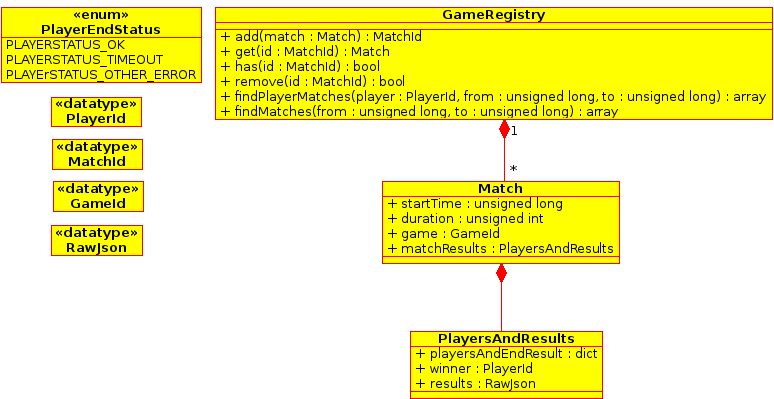
\includegraphics[scale=0.6]{./class_diagram.png}
  % class_diagram.png: 0x0 pixel, 300dpi, 0.00x0.00 cm, bb=
 \end{center}


\section{Arquitectura del sistema}
\begin{figure}[center]
 \missingfigure{TODO}
 \caption{Modelo de despliegue del sistema}
 \label{fig:arquitectura}
\end{figure}


% Tercera iteración (capítulo)
\chapter{Iteración 3}
\section{Objetivos de iteración}
\begin{itemize}
  \item Integración de Gradle 
  \item Servidor dockerizado
  \item Estructura inicial del Cliente vertx.
\end{itemize}

% Cuarta iteracion
\chapter{Iteración 4}
\section{Objetivos de iteración}
\begin{itemize}
  \item Integración de MondoDB (como contenedor docker) 
  \item Cliente más avanzado. Servidor estructurado en Servicio / Controlador.
\end{itemize}

\subsection{Distinción de dominio, controlador y servicio}
\begin{description}
  \item[Dominio] \hfill \\
  POJO clases con la misma esquema de la base de datos.
  \item[Controlador] \hfill \\
  Manejar los requisitos y respuestas y comunicar con el servicio.
  \item[Servicio] \hfill \\
  La lógica de negocio. Almacenar los sessiones en el base de datos.
\end{description}

\chapter{Iteracion 5}
\section{Objetivos de iteración}
\begin{itemize}
  \item Implementación inicial de API
  \item Primeros tests. 
  \item ¿Integración contínua?
\end{itemize}

\chapter{Iteracion 6}
\section{Objetivos de iteración}
Final testing.

\chapter{Iteracion 7}
\section{Objetivos de iteración}
Subir a repositorio Maven.

\end{document}
\appendix

\chapter{Documentación de API MyService}

Aquí el texto que se considere necesario.
